In this chapter, we will cover the basics of how sourdough ferments.
First, we will look at the enzymatic reactions that take place
in your flour the moment you add water, triggering the fermentation
process. Then, in order to understand this process better, we will
learn more about the yeast and bacterial microorganisms involved.

\begin{figure}[!htb]
  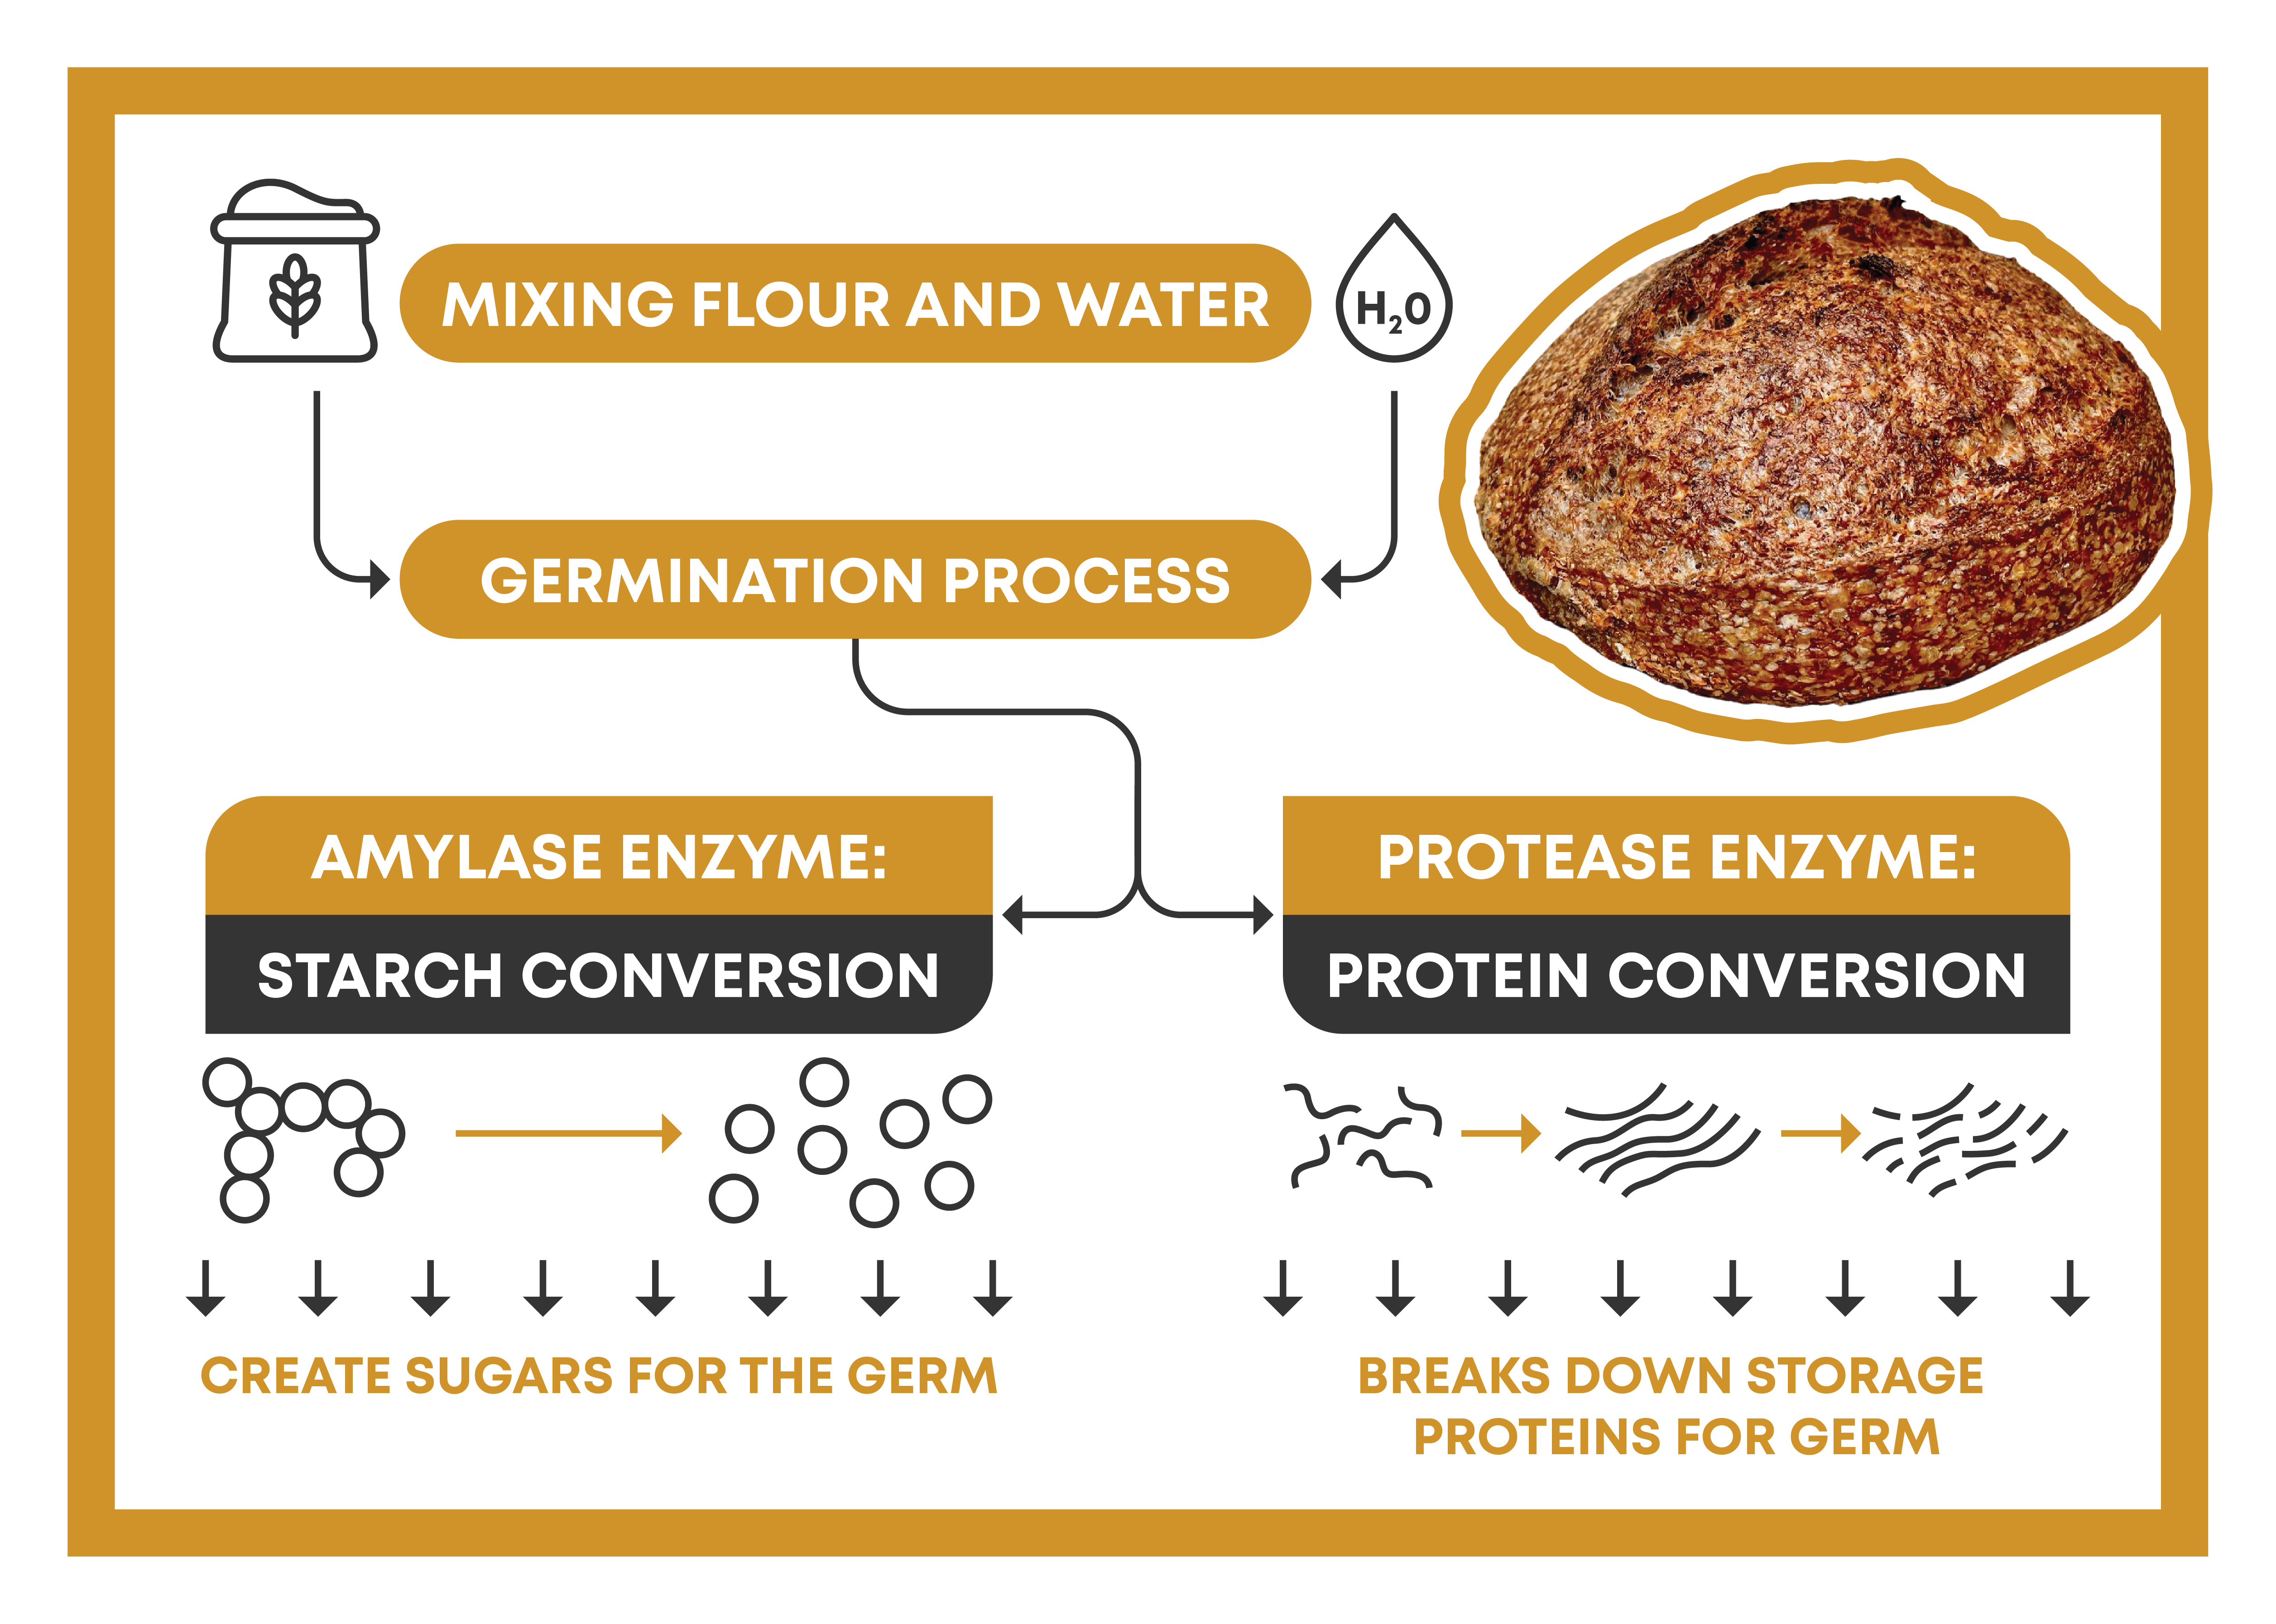
\includegraphics[width=\textwidth]{infographic-enzymes}
  \caption{How amylases and proteases interact with flour.}%
  \label{infographic-enzymes}
\end{figure}

\section{Enzymatic reactions}

To understand the many enzymatic reactions that take place when flour
and water are mixed, we must first understand seeds and their role in
the lifecycle of wheat and other grains.

Seeds are the primary means by which many plants, including wheat,
reproduce. Each seed contains the embryo of another plant, and must
therefore contain all the nutrients that new plant requires to grow.

When the seed is dry, it is in hibernation mode and can sometimes be
stored for several years. The moment it comes into contact with water,
however, it begins to sprout. The seed turns into a germ, requiring the
stored nutrients to be converted into something the plant can use while
it grows. The catalyst that makes the associated reactions possible is water.

The seed typically contains the first prototypical leaves of the plant,
and it can put down roots using the stored nutrients inside. Once those leaves
break through the soil and come into contact with the sunlight above, they
begin to photosynthesize. This process is the plant's engine, and with the
energy photosynthesis produces, the plant can continue to grow more roots,
enabling it to access additional nutrients from the soil. These additional
nutrients allow the plant to grow more leaves, increasing its photosynthetic
activity so that it can thrive in its new environment.

Of course, a ground flour can no longer sprout. But the enzymes that
trigger this process are still present. That's why it's important not to
mill grains at too high a temperature, as doing so could damage some of
these enzymes.

Normally, the grain seed shields the germ against pathogens. However, as the
grain is ground into flour, the contents of the seed are exposed. This is ideal
for our sourdough microorganisms.

Neither the yeast nor the bacteria can prepare their own food. However, as
the enzymes are activated, the food they need becomes available, allowing them
to feed and multiply.

The two main enzymes involved in this process are \emph{amylase} and
\emph{protease}. For reasons that will soon be made clear, they are of the
utmost importance to the home baker, and their role in the making of sourdough
is a key puzzle piece to making better-tasting bread.

\subsection{Amylase}

Sometimes, when you chew on a potato or a piece of bread for a long period
of time, you'll perceive a sweet flavor on your tongue. That's because your
salivary glands produce amylase. Amylase breaks down complex starch molecules
into easily-digestible sugars. Your body uses amylase to start the digestive
process. The germ works similarly by using the same enzyme. The amylase
is used to create sugars out of the starch to then produce more plant matter.

Normally,
the microorganisms on the surface of the grain can't consume the freed maltose
molecules, which remain hidden inside the germ. But as we grind the flour, a
feeding frenzy takes place. Generally, the warmer the temperature, the faster
this reaction occurs. That's why a long fermentation is key to making great
bread. It takes time for the amylase to break down most of the starch into
simple sugars, which are not only consumed by the yeast but are also essential
to the \emph{Maillard reaction}, responsible for enhanced browning during the
baking process.

If you're a hobby brewer, you'll know that it's important to keep your beer at
certain temperatures to allow the different amylases to convert the contained
starches into sugar~\cite{beer+amylase}. This process is so important that
there's a frequently used test to determine whether or not all the starches
have been converted.

This test, called the \emph{Iodine Starch Test}, involves mixing iodine into
a sample of your brew and checking the color. If it's blue or black, you know
you still have unconverted starches. I~wonder if such a test would also work
for bread dough?

Industrial bakers that add especially active yeast to produce bread in a short
period of time face a similar issue. Their approach is to add malted flour to
the dough. The malted flour contains many enzymes and thus speeds up the
fermentation process. The next time you're at the supermarket, check the
packaging of the bread you buy. If you find \emph{malt} in the list of
ingredients, chances are this strategy was used.

Note that there are actually two categories of malt. One is \emph{enzymatically
active malt}, which has not been heated to above  \qty{70}{\degreeCelsius}, where the amylases begin
to degrade. The other is \emph{inactive malt}, which has been heated to higher
temperatures and thus has no impact on your flour.

\subsection{Protease}

Just as amylase breaks starches down into simple sugars, protease breaks
complex proteins down into simpler proteins and amino acids. Because wheat
contains gluten, a protein that's essential to the structure of bread,
protease necessarily plays a crucial role in the baking of sourdough.

Since the grain seeds require smaller amino acids to build roots and other
plant materials, the gluten in those seeds will begin to break down the moment
they sprout, and since adding water to flour activates those same enzymes,
the same process occurs in bread dough.

If you've ever tried to make a wheat-based dough and kept it at room
temperature for several days, you'll have discovered for yourself that the
gluten network breaks down so that the dough can no longer hold together. Once
this happens, the dough easily tears, holds no structure, and is no
longer suitable for baking bread.

This happened to me once when I~tried to make sourdough directly from a dried
starter. At three to four days, the fermentation speed was so slow that the
gluten network broke down. The root cause for this issue was protease.

By adding water to your dough, you activate the protease, and this gets to work
in readying amino acids for the germ.

Here's another interesting experiment you can try to better visualize the
importance of protease: Make a fast-proofing dough using a large quantity
of active dry yeast. In 1--2~hours, your dough should have leavened and
increased in size. Bake it, then examine the crumb structure. You should see
that it's quite dense and nowhere near as fluffy as it could have been. That's
because the protease enzyme wasn't given enough time to do its job.

At the start, while kneading, a dough becomes elastic and holds together very
well. As that dough ferments, however, it becomes more loose and
extensible~\cite{protease+enzyme+bread}. This is because some of the gluten
bonds have
been broken down naturally by the protease through a process known as
\emph{proteolysis}. This is what makes it easier for the yeast to inflate the
dough, and it's why a long fermentation process is critical when you want to
achieve a fluffy, open crumb with your sourdough bread.

Aside from using great ingredients, the slow fermentation process is one of the
main reasons Neapolitan pizza tastes so great: because the protease creates an
extensible, easy-to-inflate dough, a soft and airy edge is achieved.

Because the fermentation process typically takes longer than 8~hours, a
flour with a higher gluten content should be used. This gives the dough more
time to be broken down by the protease without negatively affecting its
elasticity. If you were to use a weaker flour, you might end up with a dough
that's broken down so much that it tears during stretching, making it
impossible, for example, to shape it into a pizza pie.

Traditionally, pizza has been made with sourdough, but in modern times it is
made with active dry yeast, as the dough stays good for a longer period of time
and is much easier to handle on a commercial scale. If you were to use
sourdough, you might have a window of thirty to ninety minutes before the dough
begins to deteriorate, both because of the protease acting for a longer period
of time and the byproducts of bacteria, which we'll discuss in more detail later
in this chapter.

\subsection{Improving enzymatic activity}

As explained previously, malt is a common trick used to speed up enzymatic
activity. Personally, however, I~prefer to avoid malt and instead use a
trick I~learned while making whole-wheat breads.

When I~first started making whole-wheat bread, I~could never achieve the
crust, crumb, or texture I~desired no matter what I~tried. Instead, my dough
tended to overferment rather quickly. When using a white flour with a similar
gluten content, however, my bread always turned out great.

At the time, I~utilized an extended autolyse, which is just a fancy word for
mixing flour and water in advance and then letting the mixture sit. Most
recipes call for it as the process gives the dough an enzymatic head start, and
in general it's a great idea. However, as an equally effective alternative,
you could simply reduce the amount of leavening agent used (in the case of
sourdough, this would be your starter). This would allow the same biochemical
reactions to occur at roughly the same rate without requiring you to mix your
dough several times. My whole wheat game improved dramatically after I~stopped
autolysing my doughs.

Now that I've had time to think about it, the result I~observed makes sense.
In nature, the outer parts of the seed come into contact with water first, and
only after penetrating this barrier would the water slowly find its way to the
center of the grain. The seed needs to sprout first to outcompete other nearby
seeds, requiring water to enter quickly. Yet the seed must also defend itself
against animals and potentially hazardous bacteria and fungi, requiring some
barrier to protect the embryo inside. A way for the plant to achieve both goals
would be for most of the enzymes to exist in the outer parts of the hull. As a
result, they are activated first~\cite{enzymatic+activity+whole+wheat}. Therefore, by just adding a
little bit of whole flour to your dough, you should be able to significantly
improve the enzymatic activity of your dough. That's why, for plain white flour
doughs, I~usually add 10\textendash20\% whole-wheat flour.

\begin{figure}
  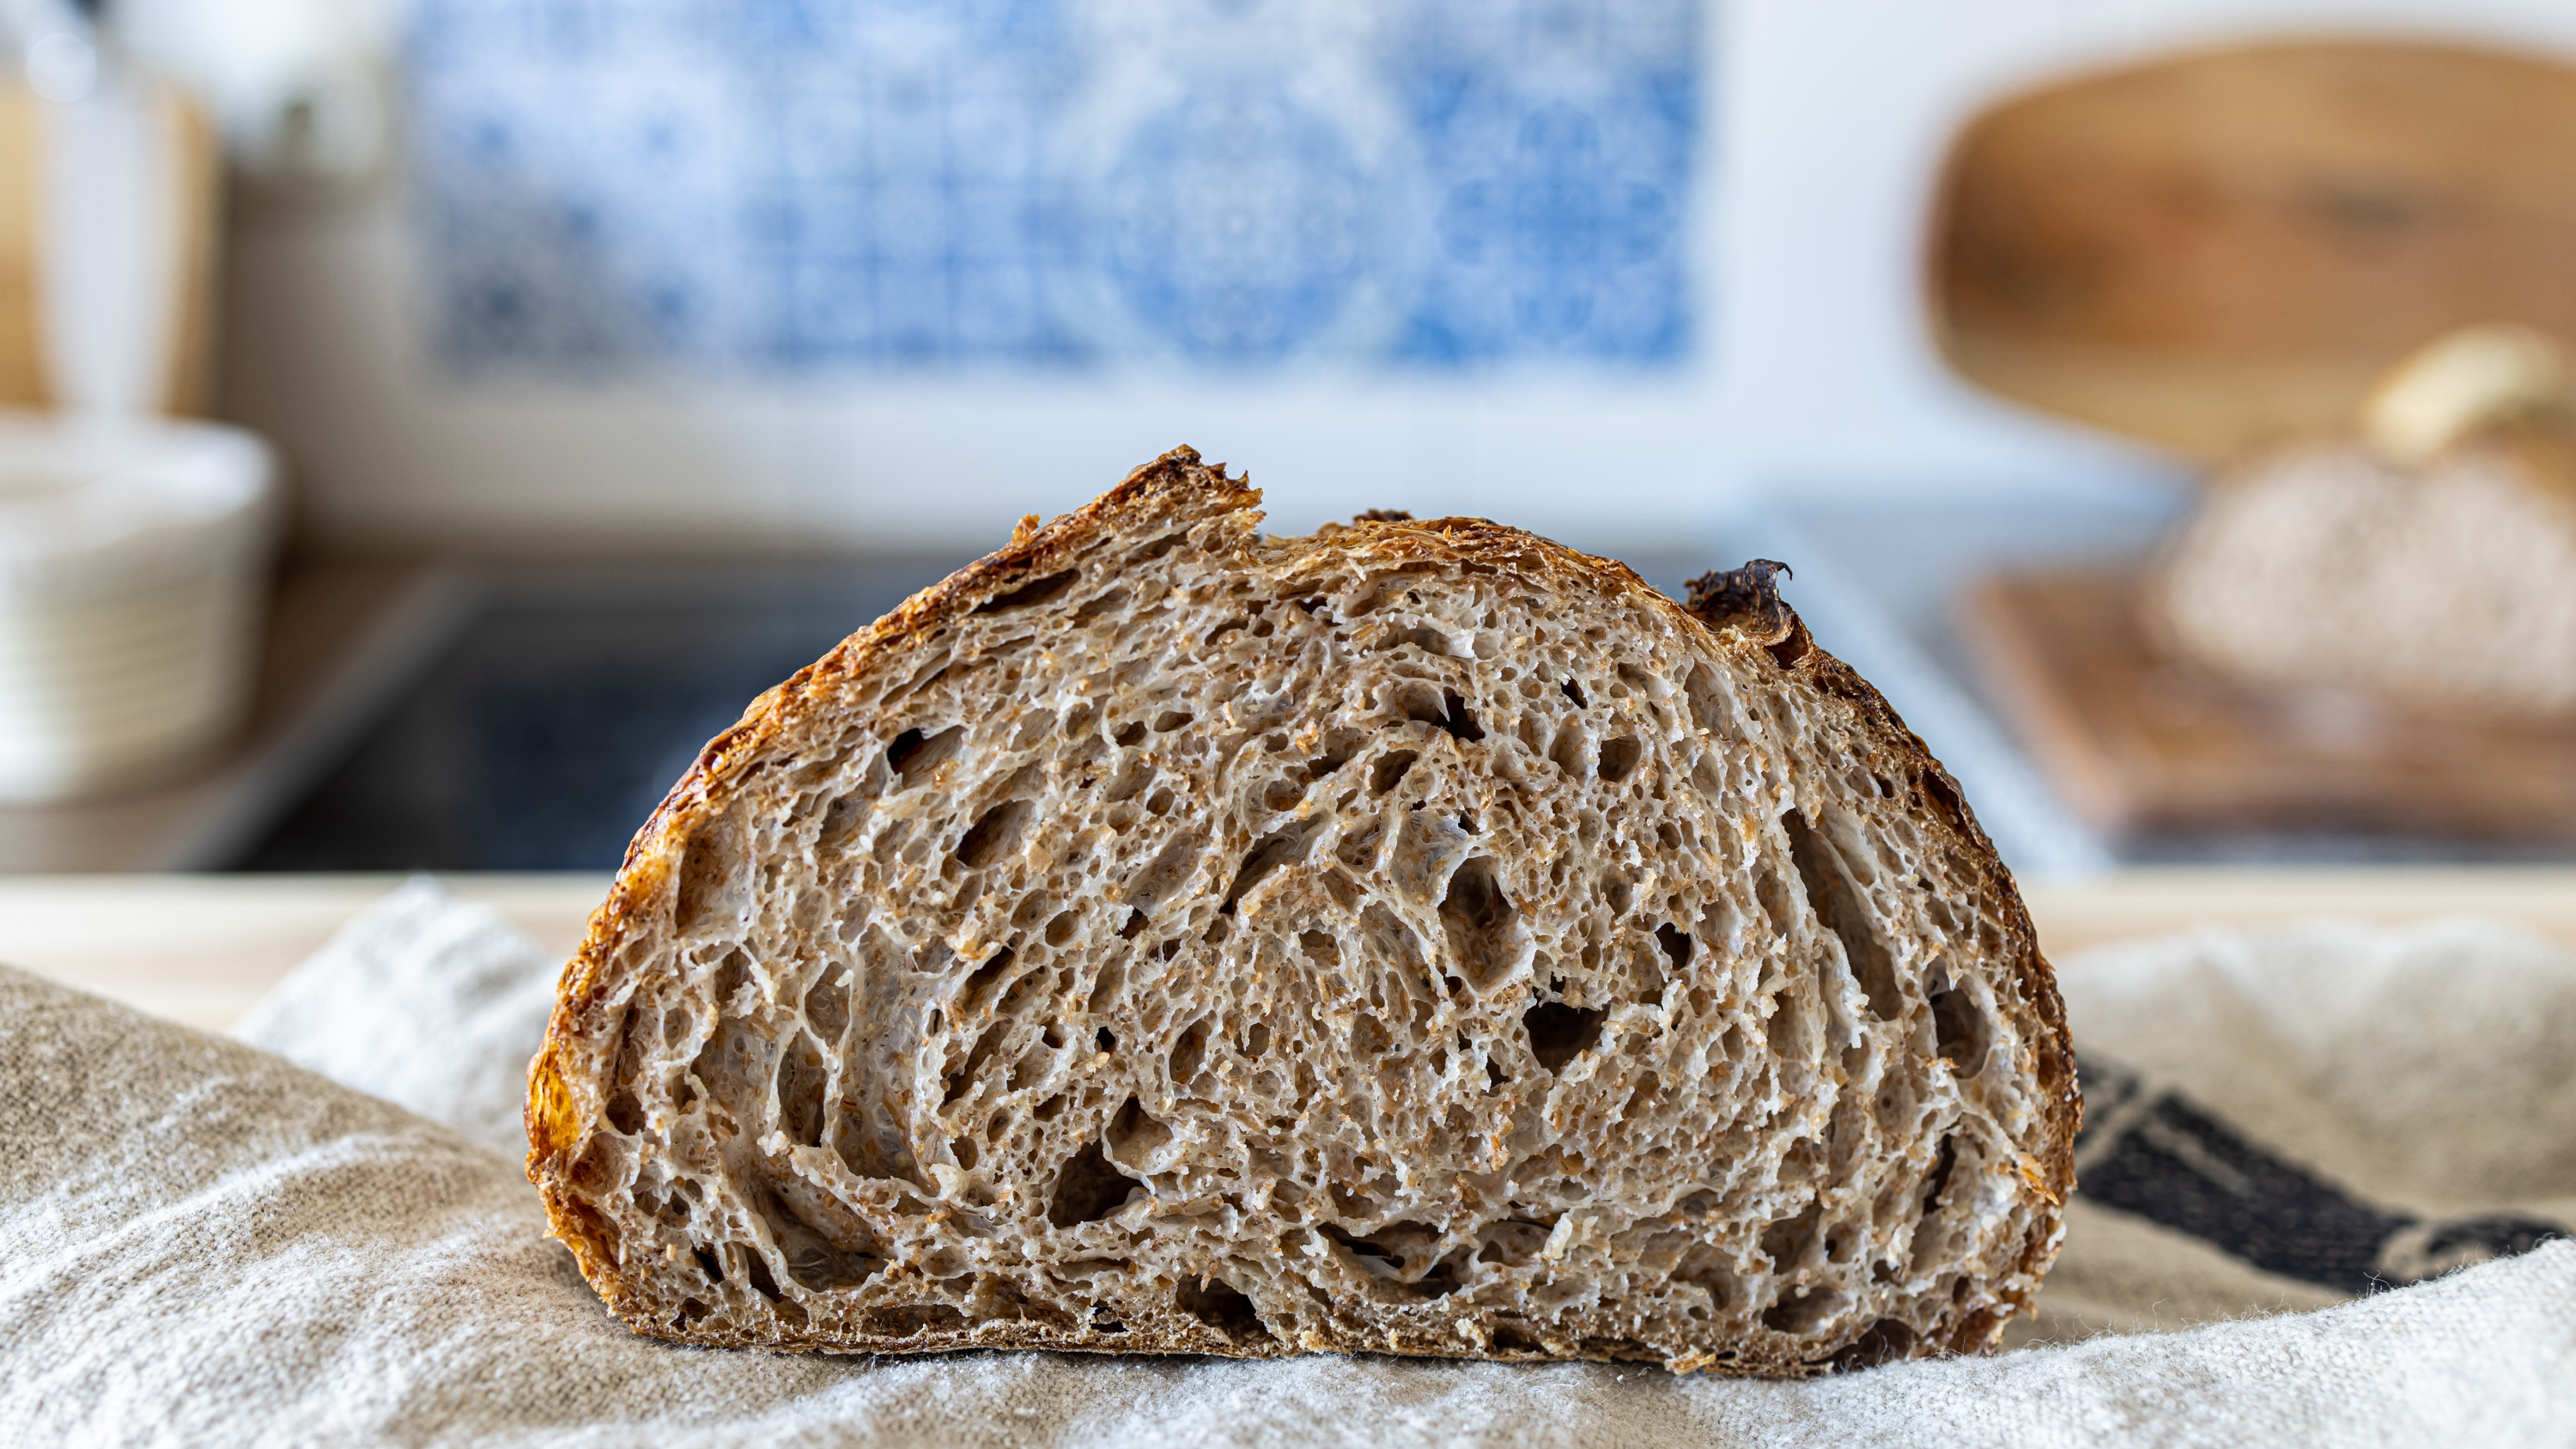
\includegraphics[width=\textwidth]{whole-wheat-crumb}
  \caption{A whole-wheat sourdough bread.}%
  \label{whole-wheat-crumb}
\end{figure}


By understanding the two key enzymes \emph{amylase} and \emph{protease}, you
will be better equipped to make bread to your liking. Do you prefer a softer
or stiffer crumb? Do you desire a lighter or darker crust? Do you wish to reduce
the amount of gluten in your final bread? These are all factors that you can
tweak just by adjusting the speed of your dough's fermentation.

\section{Yeast}

Yeasts are single-celled microorganisms belonging to the fungi kingdom, and
spores that are hundreds of millions of years old have been identified by
scientists. There are a wide variety of species --- so far, about \num{1500} have been
identified. Unlike other members of the fungi kingdom such as mold, yeasts do
not ordinarily create a mycelium network~\cite{molecular+mechanisms+yeast}.\footnote{For
one interesting exception, skip ahead to the end of this section.}

\begin{figure}[!htb]
\begin{center}
  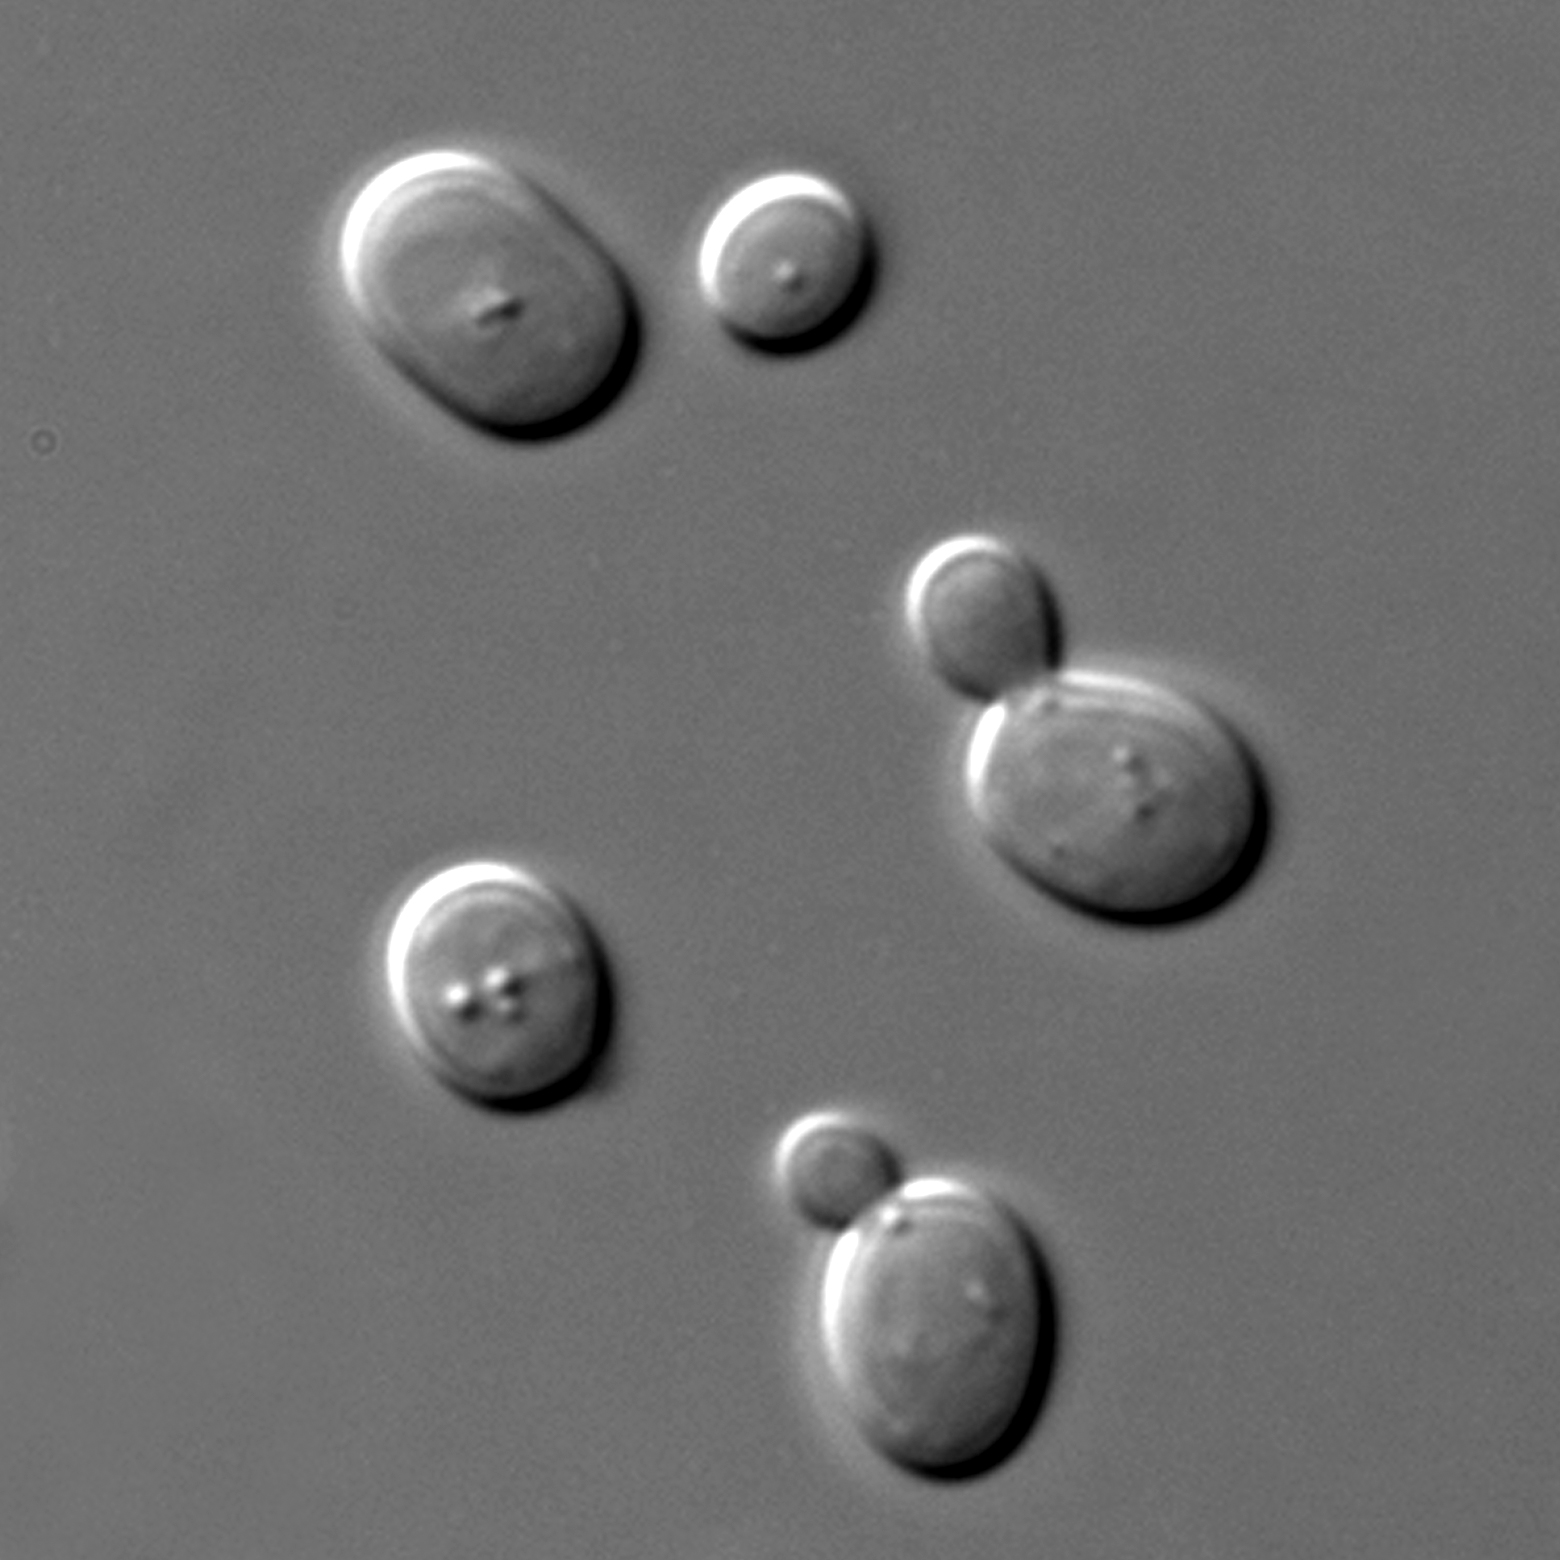
\includegraphics[width=1.0\textwidth]{saccharomyces-cerevisiae-microscope}
  \caption{Saccharomyces cerevisiae: Brewer's yeast under the microscope.}%
  \label{saccharomyces-cerevisiae-microscope}
\end{center}
\end{figure}

Yeasts are saprotrophic fungi. This means that they do not produce their own
food, but instead rely on external sources that they can decompose and break
down into compounds that are more easily metabolized.

Yeast breaks down carbohydrates into carbon dioxide and alcohol in what we today
refer to as the fermentation process. This process has been known for thousands
of years and has been used since ancient times for the making of bread as well
as alcoholic beverages.

Yeast can grow and multiply under both aerobic and anaerobic conditions. When
oxygen is present, they produce carbon dioxide and water almost exclusively.
When oxygen is not present, their metabolism changes to produce alcoholic
compounds~\cite{effects+oxygen+yeast+growth}.

The temperatures at which yeast grows varies. Some yeasts, such as
\emph{Leucosporidium frigidum}, do best at temperatures ranging from \qty{-2}{\degreeCelsius} to
 \qty{20}{\degreeCelsius}, while others prefer higher temperatures. In general, the warmer the
environment, the faster the yeast's metabolism. The variety of yeast
that you cultivate in your sourdough starter should work best within the range
of temperatures where the grain was grown and harvested. So, if you are from a
cooler place and cultivate a sourdough starter from a nordic rye variety,
chances are your yeast will prefer a colder environment.

As an example, beer makers discovered a beneficial yeast living in the cold
caves around the city of Pilsen, Czech Republic. This yeast has since become
known for producing excellent beers at lower temperatures and varieties of
these strains are now used for brewing popular lagers.

Yeasts in general are very common organisms. They can be found on cereal
grains, fruits, and many other plants in the soil. They can even be found
inside your gut! As it happens, the types of yeast we use for baking are
cultivated on the leaves of plants, though very little is known about the
ecology involved.

Plants are protected by thick cell walls that few fungi or bacteria can
penetrate. However, there are some species that produce enzymes capable of
breaking down those cell walls so they can infect the plant.

Some fungi and bacteria live inside plants without causing them any distress.
These are known as \emph{endophytes}. Not only do they \emph{not} damage their
host, they actually live in a symbiotic relationship, helping the plants in
which they dwell to protect themselves from other pathogens that might also
come to infect them through their leaves. In addition to this protection, they
also help with water and heat stress, as well as the availability of nutrients.
In exchange for their service to their host plants, these fungi and bacteria
receive carbon for energy.

However, the relationship between endophyte and plant is not always mutually
beneficial, and sometimes, under stress, they become invasive pathogens and
ultimately cause their host to decay~\cite{endophytes+in+plants}.

There are other microorganisms that, unlike endophytes, do not penetrate cell
walls but instead live on the plant's surface and receive nutrients from rain
water, the air, or other animals. Some even feed on the honeydew produced by
aphids or the pollen that lands on the surface of the leaves. Such organisms
are called \emph{epiphytes}, and included among them are the types of yeast
we use for baking.

Interestingly, when you remove external food sources, a large number of
epiphytic fungi and bacteria can still be found on the plant's surface,
suggesting that they must somehow be feeding directly from the plant.
Indeed, there is some research indicating that some plants intentionally release
compounds such as sugars, organic and amino acids, methanol, and various
salts along the surface. These nutrients would then attract the epiphytes that
live on the plant's surface.

Epiphytes are advantageous to a plant's survival, as they are provided with
enhanced protection against mold and other pathogens. Indeed, it is in the
best interest of the epiphytes to keep their host plants alive for as long as
possible~\cite{leaf+surface+sugars+epiphytes}.

More research is conducted every day into ways that yeasts can be used as
biocontrol agents to protect plants, the advantage being that these bio-agents
would be food-safe as the relevant strains of yeast are generally considered
harmless to humans. The yeasts would grow and multiply on the leaves,
essentially shielding them from other types of mold. This could be a potential
game changer for vineyards that suffer from mildew.

Such bio-agents could also be used to shield plants against the psychoactive
ergot fungus, which likes to grow in colder, more humid environments and
poses a significant problem for rye farmers.
Lawmakers have recently reduced the amount of allowed ergot contamination in
rye flour because it infects the grain and makes it unfit for consumption due
to its high toxicity to the liver. Yeasts could help to mitigate ergot contamination.

There is another interesting experiment performed by Italian scientists that
shows how crucial yeasts could be in protecting our crops. First, they made
tiny incisions into some of the grapes on a vine. Then, they infected the
wounds with mold. Some incisions were only infected with mold. Others were also
inoculated with some of the 150 different wild yeast strains isolated from the
leaves. They found that when the wound was inoculated with yeast, the grape
sustained no significant damage~\cite{yeasts+biocontrol+agent}.

Intriguingly, there was also an experiment performed that showed how brewer's
yeast could function as an aggressive pathogen to grapevines. Initially, the
yeast lived in symbiosis with the plants, but after the vines sustained heavy
damage, the yeast became opportunistic and started to attack, even going so far
as to produce hyphae, the mycelium network normally associated with a fungus,
so that they could penetrate the tissue of the plants.

\section{Bacteria}

The other most dominant microbial antagonists in your sourdough are bacteria.
In fact, they are so dominant that they outnumber the yeast in your dough 100
to 1. Whereas yeast provides leavening power, bacteria create the distinct
flavours for which sourdough has been named. These are due to the acidic
byproducts that result from bacterial feeding. As a bonus, these acids
can significantly increase the shelf life of sourdough
breads~\cite{shelflife+acidity}.

\begin{figure}
  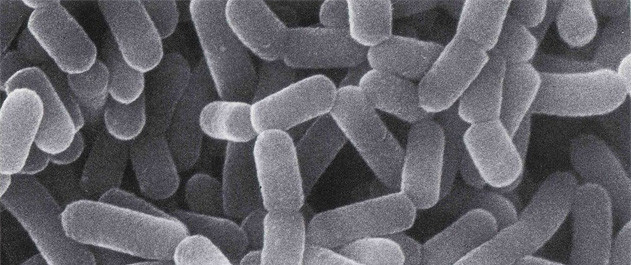
\includegraphics[width=1.0\textwidth]{bacteria-microscope}
  \caption{Fructilactobacillus Sanfranciscensis under the microscope.}%
  \label{lactobacillus-franciscensis-microscope}
\end{figure}

There are two predominant types of acid produced in sourdough bread: lactic and
acetic. In terms of flavor, lactic acid has clear dairy notes, while acetic
acid tastes of vinegar (of which it is, in fact, the primary ingredient!). These
acidic byproducts are produced by both \emph{homofermentative} and
\emph{heterofermentative} lactic acid bacteria.

\emph{Homofermentative} means that, during fermentation, the bacteria produce
a single compound: in this case, lactic acid. \emph{Heterofermentative}, on
the other hand, means that other compounds are also produced: in this case,
not only lactic acid, but also acetic acid, as well as ethanol and even some
carbon dioxide, two byproducts ordinarily associated with yeast. One quite
famous strain of lactic acid bacteria, \emph{Fructilactobacillus sanfranciscensis},
derives its name from the equally famous San Francisco style sourdough bread.
The first isolated culture came from a bakery in this city, hence the name.

Yeast and bacteria both compete for the same food source: sugar. Some scientists
have reported that bacteria consume mostly maltose, while yeast prefer glucose.
Others have reported that bacteria feed on the byproducts of yeast and vice
versa. This makes sense, as nature generally does a superb job of composting
and breaking down biological matter~\cite{lactobacillus+sanfrancisco}.

I~have yet to find a proper source that clearly describes the symbiosis between
yeast and bacteria, but my current understanding is that they both coexist and
sometimes benefit each other, but not always. Yeast, for example, tolerate the
acidic environment created by the surrounding bacteria and are thus protected
from other pathogens. Meanwhile, however, other research demonstrates that both
types of microorganisms produce compounds that prevent the other from
metabolizing food --- an interesting observation, by the way, as it could help to
identify additional antibiotics or fungicides~\cite{mold+lactic+acid+bacteria}.

In the past, I've tried cultivating mushrooms and observed the mycelium
attempting to defend itself against the surrounding bacteria; both types of
microorganisms actively produced compounds to combat each other. And yet,
after a while, the fight seemed to reach a standstill, as the mycelium had
fully grown around the bacterial patch, preventing it from spreading further.
I~imagine a similar scenario could be playing out in our sourdough starters,
although, given that the sourdough environment tends to be more liquid, this
fight would have to take place everywhere in the dough and not just in an
isolated patch. More research on this topic is required to get a better understanding of
the details of the relationship between yeast and bacteria.


One other interesting trait of sourdough bacteria worth mentioning is their
ability to break down and consume the proteins in your dough. If you've baked
sourdough before, chances are you've experienced this firsthand. You'll recall
from the \emph{Enzymatic reactions} section that protease breaks down the
gluten network in your dough, resulting in a sticky mess if left unbaked for
too long. The bacteria, too, consume and break down the gluten in your
dough through a process called \emph{proteolysis}.

This, to me, was a great riddle when I~first started working with sourdough.
On the one hand, it makes the dough stickier. On the other, it makes the dough
more extensible and easier to work with. As the gluten is reduced, the dough
becomes easier for the microorganisms to inflate, allowing it to rise. This
could be likened to the level of effort required to inflate a thick rubber tire
versus a thin and fragile balloon. The latter would be easy to blow up with
your mouth, while the former would not.

Unsurprisingly, proteolysis is further accelerated by the protease enzyme
previously discussed, which aids in the breakdown of gluten into smaller,
more easily metabolized amino acids.

This, to me, is the amazing process of fermentation. When you eat sourdough
bread, you are not merely consuming flour and water but the end result of
complex biological processes accomplished by the bacteria and yeast. Because
of the added bacterial component, sourdough bread typically contains less
gluten than a pure yeast-based dough~\cite{proteolysis+sourdough+bacteria}.
Furthermore, the homofermentative bacteria metabolize the ethanol produced by
the yeast and other heterofermentative lactic acid bacteria. In both cases,
most of the resulting compounds are organic acids. Every natural resource in
your sourdough bread is recycled by the microorganisms inside, which are all
trying to eat whatever is available for as long as possible, and with each
feeding, they become more adept at utilizing these resources.

Depending on which flavour profile you prefer, you can select for one organic
acid or another. Acetic acid production requires oxygen, and by depriving
your sourdough starter of it, you can boost the population of homofermentative
lactic acid bacteria. Over time they will become dominant and outcompete the
acetic acid-producing bacteria~\cite{acetic+acid+oxygen}.

The optimal fermentation temperature of your lactic acid bacteria depends on
the strains you've cultured in your starter. Generally, they work best at the
temperature used to create your starter because you've already selected for
bacteria that thrive under that condition.

In one noteworthy experiment, scientists examined the lactic acid bacteria
found on corn leaves. They lowered the ambient temperature from \qtyrange{20}{25}{\degreeCelsius} to around
\qtyrange{5}{10}{\degreeCelsius} and afterward observed varieties of the bacteria that had never been
seen before~\cite{temperature+bacteria+corn}, confirming that there is, in
fact, a large variety of bacterial strains living on the leaves of the plant.

Incidentally, you could perform a similar experiment by kicking off a sourdough
starter at a lower temperature. In theory, the microbiome should adapt, as the
microorganisms that thrive the most at lower temperatures will start to become
dominant. It would be interesting to see if this could actively influence the
taste of the resulting bread.

One last footnote worth mentioning: Some sources say that fermenting at a
lower temperature can increase acetic acid production, while fermenting at a
warmer temperature can boost lactic acid production. I~could not verify this
in my own tests. More research is needed on the topic.
